
The pdf is given by
\begin{align}
    f_{X}(x) = \frac{1}{2\pi} \int_{-\infty}^{\infty}  \phi_{X}\brak{t}e^{-jxt} dt 
\end{align}
If
\begin{align}
    g\brak{x} &\system{F} G\brak{t}\\
    \implies G\brak{t} &\system{F} g\brak{-x} \label{st2020-16:th}
\end{align}
where $ \brak{\system{F}}$ represents Fourier transform and
\begin{align}
    G\brak{t}  = \int_{-\infty}^{\infty} g\brak{x} e^{-j2\pi xt} dx 
\end{align}
we know that the Fourier transform of rectangular function is sinc function
\begin{align}
    rect\brak{\frac{x}{\tau}} &\system{F} \tau sinc(t\tau)
\end{align}
from \eqref{st2020-16:th} we get
\begin{align}
  \tau sinc(t\tau) &\system{F} rect\brak{-\frac{x}{\tau}}
\end{align}
\begin{align}
 \implies rect\brak{-\frac{x}{\tau}} = \int_{-\infty}^{\infty} \tau \frac{\sin{\pi t \tau}}{{\pi t \tau}} e^{-j2\pi xt}dt
\end{align}
substituting $\tau = \frac{2}{\pi}$ and changing $2\pi x \rightarrow x $ we get
\begin{align}
    \frac{1}{4}rect\brak{\frac{-x}{4}} = \frac{1}{2\pi} \int_{-\infty}^{\infty} \brak {\frac{\sin{2t}}{2t}}e^{-jxt} dt 
\end{align}
So
\begin{align}
    f_{X}(x) &= \frac{1}{4}rect\brak{\frac{-x}{4}}\\
    P\brak{|X|\leq \frac{3}{2}} &= \int_{\frac{-3}{2}}^{\frac{3}{2}} \frac{1}{4} dx\\
    &=\frac{3}{4}
\end{align}
\begin{figure}[!ht]
\centering
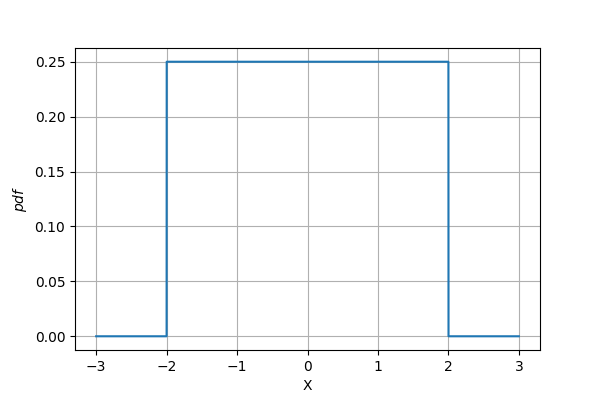
\includegraphics[width=\columnwidth]{solutions/st/2020/16/figs/Assignment5.png}
\caption{$f_{X}(x)$}
\label{st2020-16:pdf}
\end{figure}


